\documentclass[a4paper]{article}
\usepackage[english]{babel}
\usepackage[utf8]{inputenc}

%
% Graphics
%
\usepackage{graphicx}
\usepackage{xcolor}

\definecolor{alpha}{HTML}{3FA9F5}

%
% Bibliography
%
\usepackage[backend=bibtex,maxnames=5,sorting=none,url=false]{biblatex}
\usepackage{csquotes}

%
% Listings
%
\usepackage{listings}

\definecolor{background}{HTML}{FAFAFA}
\definecolor{sign}{HTML}{3FA9F5}

\lstdefinelanguage{fortune}{
  basicstyle=\ttfamily,
  basewidth={0.5em,0.5em},
  backgroundcolor=\color{background},
  literate=
   *{\%}{{{\color{alpha}{\%}}}}{1}
}

\lstdefinelanguage{shell}{
  basicstyle=\ttfamily,
  basewidth={0.5em,0.5em},
  backgroundcolor=\color{background},
  literate=
    [*]{\\\$}{{{\color{alpha}{\$}}}}{1}
       {Command>}{{{\color{alpha}{Command>}}}}{8}
       {ivan(0)>}{{{\color{alpha}{ivan(0)>}}}}{8}
       {ivan(1)>}{{{\color{alpha}{ivan(1)>}}}}{8}
       {ivan(0):RELEASED>}{{{\color{alpha}{ivan(0):RELEASED>}}}}{17}
       {ivan(0):LOCKED>}{{{\color{alpha}{ivan(0):LOCKED>}}}}{15}
       {ivan(1):LOCKED>}{{{\color{alpha}{ivan(1):LOCKED>}}}}{15}
       {ivan(2):LOCKED>}{{{\color{alpha}{ivan(2):LOCKED>}}}}{15}
}

\lstdefinelanguage{json}{
  basicstyle=\ttfamily,
  basewidth={0.5em,0.5em},
  backgroundcolor=\color{background},
  literate=
   *{:}{{{\color{alpha}{:}}}}{1}
    {,}{{{\color{alpha}{,}}}}{1}
    {\{}{{{\color{alpha}{\{}}}}{1}
    {\}}{{{\color{alpha}{\}}}}}{1}
    {[}{{{\color{alpha}{[}}}}{1}
    {]}{{{\color{alpha}{]}}}}{1}
}

\lstnewenvironment{fortune}%
{\lstset{language=fortune}}%
{}

\lstnewenvironment{json}%
{\lstset{language=json}}%
{}

\lstnewenvironment{shell}%
{\lstset{language=shell}}%
{}

%
% Links
%
\usepackage{hyperref}
\hypersetup{%
  colorlinks=true,
  citecolor={alpha},
  linkcolor={alpha},
  urlcolor ={alpha}
}

%
% Text
%
\newcommand{\ie}{i.e.}
\newcommand{\eg}{e.g.}
\newcommand{\etc}{etc.}

\newcommand{\fix}{should be modified}
\newcommand{\leave}{no changes are needed}
\newcommand{\overwrite}{should contain your previous changes}

\newcommand{\python}{\texttt{Python}}
\newcommand{\classname}[1]{\texttt{#1}}
\newcommand{\filename}[1]{\texttt{#1}}
\newcommand{\code}[1]{\texttt{#1}}

%
% References
%
\newcommand{\sref}[1]{Section~\ref{sec:#1}}
\newcommand{\tref}[1]{Table~\ref{tab:#1}}
\newcommand{\fref}[1]{Figure~\ref{fig:#1}}

\newcommand{\slabel}[1]{\label{sec:#1}}
\newcommand{\tlabel}[1]{\label{tab:#1}}
\newcommand{\flabel}[1]{\label{fig:#1}}

\newcommand{\slab}[1]{\label{sec:#1}}
\newcommand{\tlab}[1]{\label{tab:#1}}
\newcommand{\flab}[1]{\label{fig:#1}}

\newcommand{\aref}[1]{Lab~#1 \cite{description#1}}


\bibliography{include/references.bib}

\title{Distributed Systems: Lab 5\\Client-Server Database with Replicas}
\author{Petru Eles and Ivan Ukhov\\
\vspace{0.5em}
\href{mailto:petru.eles@liu.se}{petru.eles@liu.se} and \href{mailto:ivan.ukhov@liu.se}{ivan.ukhov@liu.se}
}
\date{January 24, 2016}

\begin{document}
\maketitle

\section{Introduction}
\begin{figure}
  \centering
  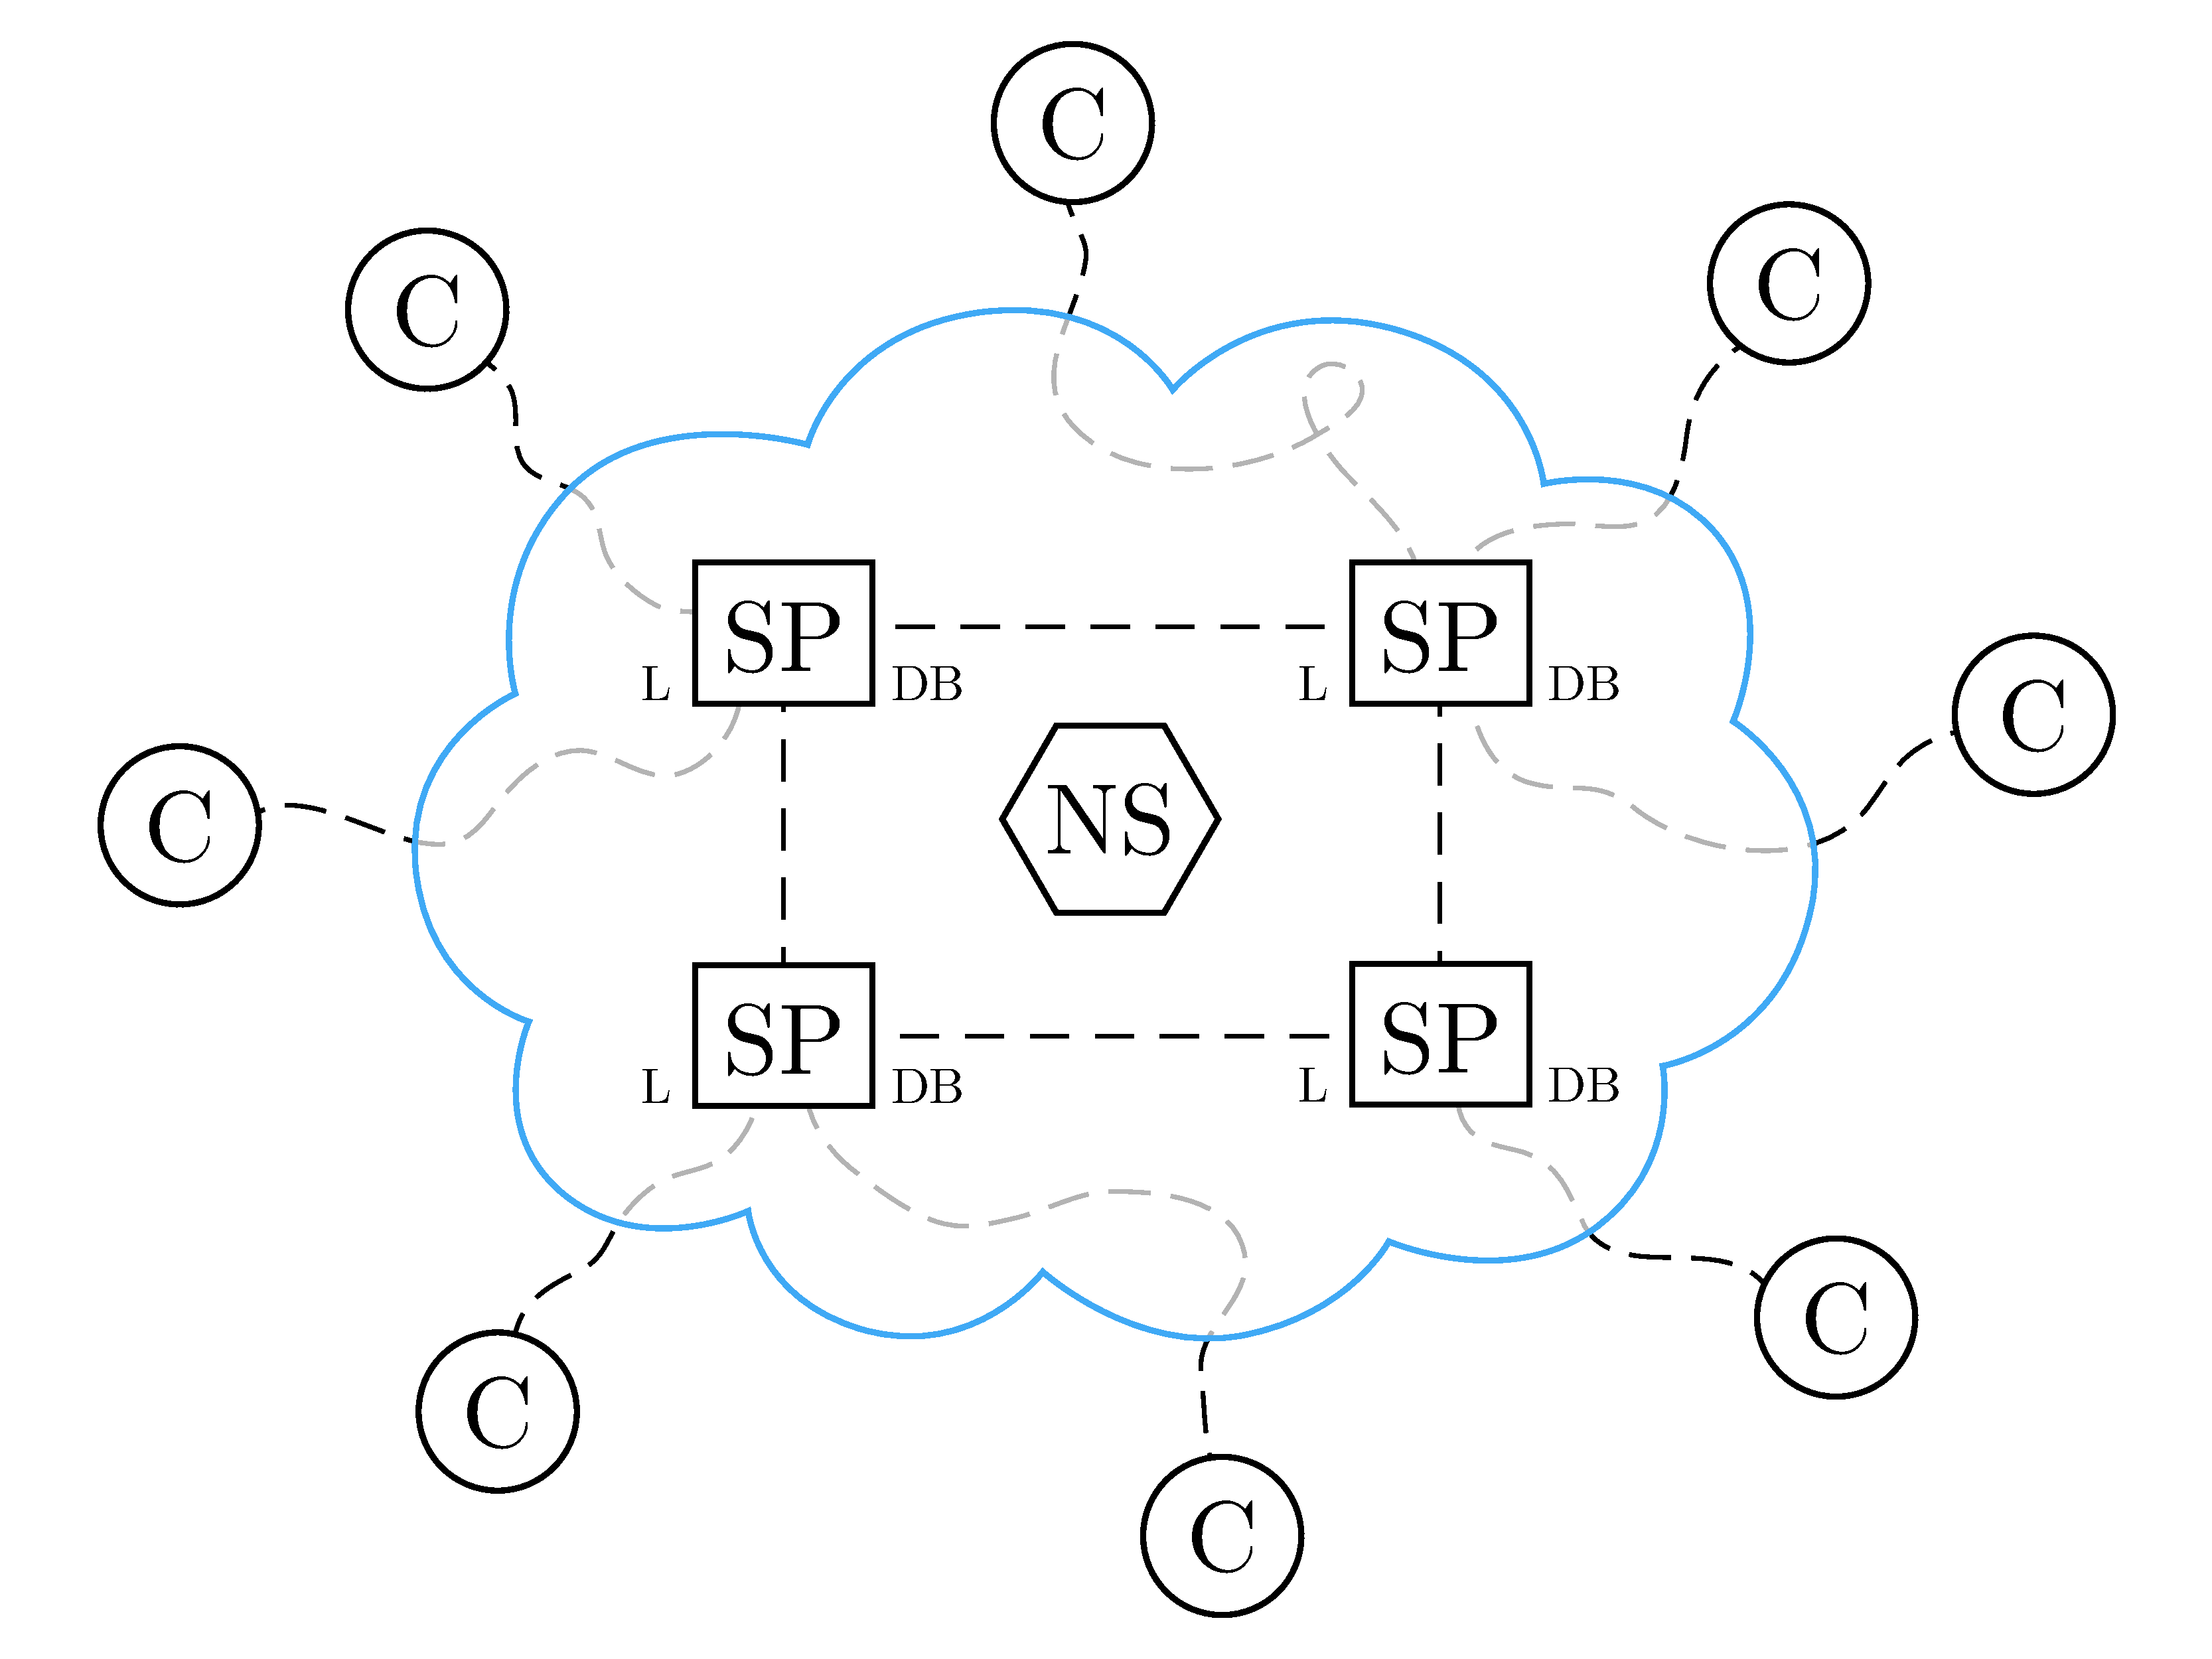
\includegraphics[width=0.8\textwidth]{include/assets/distributed-database.pdf}
  \caption{A distributed database with a number of servers/peers (SP) and a number of clients (C). Each server maintains a copy of the database (DB) protected by a distributed lock (L). The discovery process is facilitated by virtue of a name service (NS).}
  \flabel{distributed-database}
\end{figure}

Let us summarize what has been achieved so far. In the first two labs, counting
from zero, you implemented the basic functionality of a database following the
client-server model. Specifically,
\begin{itemize}

  \item the user can perform the read and write operations on the data, that is,
  read random fortunes and compose new ones (\aref{0});

  \item there is only one server machine responsible for managing the data, and
  there can be many clients that can connect to the server in order to issue the
  two possible commands (\aref{1}).

\end{itemize}
In the last three labs, from two to four, you built the core components of a
distributed system. These components are as follows:
\begin{itemize}

  \item an object request broker, which, together with the name service,
  provides a handy middleware layer for your system (\aref{2});

  \item a smart peer list, which adequately keeps track of the peers that are
  currently present in the network (\aref{3});

  \item a distributed lock, which guards shared resources from being left in
  corrupted states due to concurrent operations (\aref{4}).

\end{itemize}
The goal of this lab is to improve the na\"{i}ve database obtained at the end of
\aref{1} by fusing it with the three components of a distributed system listed
above. The target configuration of the system is displayed in
\fref{distributed-database}, in which each peer\footnote{The words \emph{peer}
and \emph{server} are used interchangeably in our context. Similarly, the words
\emph{user} and \emph{client} have the same meaning here.} maintains a copy of
the data (that is, a list of fortunes) in such a way that this copy is kept
consistent with the copies of other peers. In order to achieve this consistency,
all writing operations performed on one copy of the data (owned by one of the
peers) are to be properly propagated to all other copies (located at the rest of
the peers). Having done so, any reading operation issued by a client will be
guaranteed to see the same data regardless of the peer chosen for reading.

In the scenario described above, the peers duplicating the data are typically
referred to as replica managers. This concept is of high importance for the
current lab, and, therefore, it might be a good idea to get yourself familiar
with it before diving deeper into the lab. All the needed information on the
subject can be found in the corresponding lecture notes \cite{lecture8}. In
particular, make sure you understand the read-any/write-all protocol, which our
replica managers will be assumed to follow.

\section{Your Task}
\subsection{Preparation} \slab{preparation}
Continue working with the same code base that you have been working with so far,
including all the changes that you have made. The files relevant to this lab are
listed below. You should read and understand them.
\begin{itemize}

  \item \filename{lab5/client.py} --- the client application representing a user
  of the database (\leave);

  \item \filename{lab5/serverPeer.py} --- the server application representing a
  replica manager (\fix);

  \item \filename{lab5/test.sh} --- a shell script that you can use for testing;

  \item \filename{lab5/dbs/fortune.db} --- a text file with a list of fortunes
  (the format is described in \aref{0});

  \item \filename{modules/Common/nameServiceLocation.py} --- the same as for
  \aref{2} (\leave);

  \item \filename{modules/Common/objectType.py} --- the same as for \aref{2}
  (\overwrite);

  \item \filename{modules/Common/orb.py} --- the same as for \aref{2}
  (\overwrite);

  \item \filename{modules/Common/wrap.sh} --- the same as for \aref{1};

  \item \filename{modules/Server/database.py} --- the same as for \aref{1}
  (\overwrite);

  \item \filename{modules/Server/peerList.py} --- the same as for \aref{3}
  (\overwrite);

  \item \filename{modules/Server/lock/distributedReadWriteLock.py} --- a
  distributed version of the read/write lock given by \classname{ReadWriteLock}
  using the distributed lock given by \classname{DistributedLock} (\fix);

  \item \filename{modules/Server/lock/distributedLock.py} --- the same as for
  \aref{4} (\overwrite);

  \item \filename{modules/Server/lock/readWriteLock.py} --- the same as for
  \aref{1} (\leave).

\end{itemize}
Study the code of the two main applications given in the source files
\filename{client.py} and \filename{serverPeer.py} and try to grasp the main idea
behind the scene. It might be helpful to run the code. To this end, you need to
have at least one instance of each of the applications. Here is an example:
\begin{shell}
\$ ./serverPeer.py -t ivan
Choose one of the following commands:
    l  ::  list peers,
    s  ::  display status,
    h  ::  print this menu,
    q  ::  exit.
ivan(1)>
...
\$ ./client.py -t ivan
Connecting to server: (u'130.236.205.175', 45143)
None
\end{shell}
It is apparent that the system does not work: the replica manager, running in
one terminal window, returned \texttt{None} to the user, running in another
terminal window, despite the fact that \filename{fortune.db} is non-empty.

\subsection{Understanding the Setup}
An instance of \filename{serverPeer.py} is a server/peer that maintains a local
copy of the data and collaborates with other servers in order to keep this copy
up-to-date. An instance of \filename{client.py} is a client/user of the
distributed database that connects to one of the peers and can issue the
read/write operations via the corresponding text menu (similar to the first two
labs). A client chooses a server to connect to by virtue of the name service,
which you can easily tell by looking at the corresponding code. More
specifically, in \filename{client.py}, you can discover two new functions that
the interface of the name service has:
\begin{itemize}

  \item \code{require\_any} --- the function returns the address of a randomly
  chosen peer, that is, a randomly chosen replica manager;

  \item \code{require\_object} --- the function returns the address of a
  specific peer (in case you want to connect to a particular server for
  debugging purposes).

\end{itemize}
These functions were intentionally omitted in the description of the interface
of the name service given in \aref{2}.

Another important aspect to realize is that there two types of concurrent
accesses that might occur with respect to each peer. The first type can be
labeled as ``local,'' and it is due to the same reasons as the ones described in
\aref{1}: one server can serve several clients simultaneously in separate
threads. Consequently, the thread-safeness should still be ensured, which was
previously the job of the \classname{ReadWriteLock} class. The second type can
be labeled as ``global'' or ``distributed,'' and it is due to the fact that
another peer might try to synchronize its data with the data of the current
peer. It happens when a client connected to a peer writes a new fortune into the
local database of that peer, and this new fortune needs to be pushed into the
local databases of all other peers. Consequently, such situations should be also
properly resolved, and your \classname{DistributedLock} is in high demand in
this context.

\subsection{Implementation} \slab{implementation}
As you can see in the source code of this lab, the system has already been
assembled for you. Assuming that you have properly transfered your (hopefully
correct) implementations from the previous lab to the current one (see
\sref{preparation}), there is only one problem to solve.

Neither \classname{ReadWriteLock} nor \classname{DistributedLock} is sufficient
by itself. The former is not aware of the distributed nature of the system, and
the latter is not capable of distinguishing between read and write operations.
This leads to inefficiency, which you should be able to explain. Therefore, your
task now is to merge the two locks to produce a distributed read/write lock. The
class to look at is \classname{DistributedReadWriteLock} in
\filename{distributedReadWriteLock.py}.

Having completed \classname{DistributedReadWriteLock}, you are asked to utilize
the lock in order to finish the implementation of \filename{serverPeer.py}
following the read-any/write-all policy \cite{lecture8}. Specifically, you will
have to write two functions with rather suggestive names: \texttt{read} and
\texttt{write}.

\section{Conclusion}
Congratulations! You have successfully completed the final lab of the course. In
this lab, you have put together many of the ideas that you learned previously
and have created a robust distributed database, which is able to serve many
clients in parallel balancing the workload among several servers spread out
across the network. We hope that you enjoyed this programming project. Good
luck!

\printbibliography

\end{document}
